% !TeX spellcheck = cs_CZ
%{\tikzset{external/prefix={tikz/FYZII/}}
% \tikzset{external/figure name/.add={ch06_}{}}
%---------------------------------------------------------------------------------------------------
% file fey1ch08.tex
%---------------------------------------------------------------------------------------------------
%====================Kapitola: Použití Gaussova zákona ============================================
\chapter{Elektrostatická energie}\label{fyz:IIchapVI}
\minitoc


\section{Elektrostatická energie nábojů. Homogenní koule}\label{fyz:IIchapVIsecI}

  \begin{figure}[ht!]  %\ref{fyz:fig178}
    \centering
    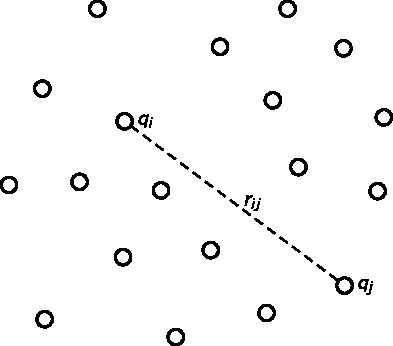
\includegraphics[width=0.7\linewidth]{fyz_fig178.pdf}
    \caption{Elektrostatická energie soustavy částic je rovna součtu elektrostatických energií 
             všech párů částic v soustavě
             (\cite[s.~140]{Feynman02}).}
    \label{fyz:fig178}
  \end{figure}
  
  \begin{figure}[ht!]  %\ref{fyz:fig179}
    \centering
    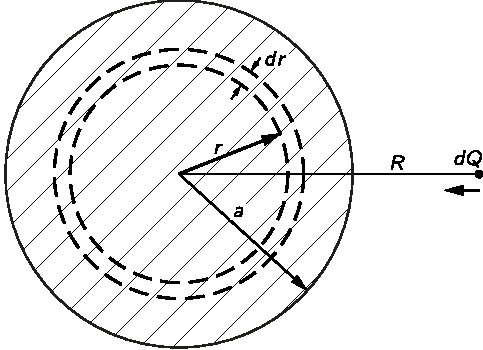
\includegraphics[width=0.7\linewidth]{fyz_fig179.pdf}
    \caption{Energii homogenně nabité koule můžeme počítat tak, že si představíme kouli, jako by 
             byla složena ze vzájemně na sebe přiléhajících kulových slupek. 
             (\cite[s.~141]{Feynman02}).}
    \label{fyz:fig179}
  \end{figure}

\section{Energie kondenzátoru. Síly působící na nabité vodiče}\label{fyz:IIchapVIsecII}

  \begin{figure}[ht!]  %\ref{fyz:fig180}
    \centering
    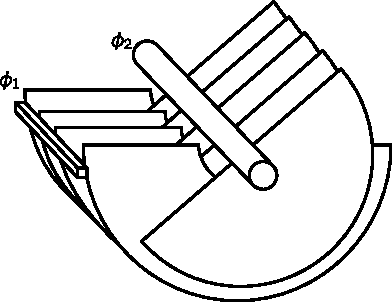
\includegraphics[width=0.7\linewidth]{fyz_fig180.pdf}
    \caption{Jaký moment síly působí na otočný kondenzátor?
             (\cite[s.~144]{Feynman02}).}
    \label{fyz:fig180}
  \end{figure}
  
  \begin{figure}[ht!]  %\ref{fyz:fig181}
    \centering
    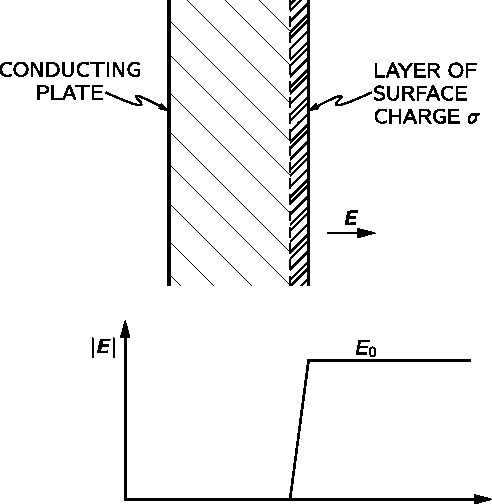
\includegraphics[width=0.7\linewidth]{fyz_fig181.pdf}
    \caption{Intenzita elektrického pole se změní při průchodu vrstvou plošného náboje existujícího 
             na povrchu vodiče z nuly na hodnotu \(E_0 = \frac{\sigma}{\varepsilon_0}\)
             (\cite[s.~145]{Feynman02}).}
    \label{fyz:fig181}
  \end{figure}
  
\section{Elektrostatická energie iontového krystalu}\label{fyz:IIchapVIsecIII}

  \begin{figure}[ht!]  %\ref{fyz:fig182}
    \centering
    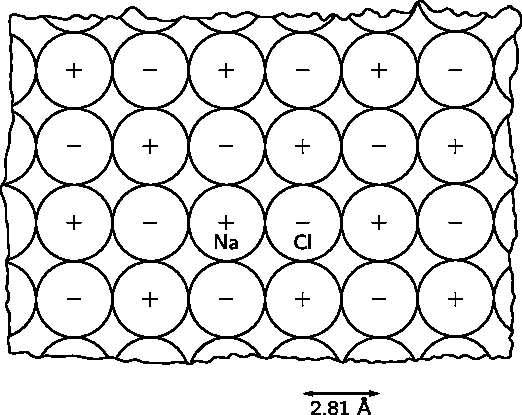
\includegraphics[width=0.7\linewidth]{fyz_fig182.pdf}
    \caption{Řez krystalem kuchyňské soli v atomovém měřítku. Šachovnicové uspořádání iontů \ce{Na} 
             a \ce{Cl} je stené v obou na sebe kolmých řezech krystalem (obr. 1.7 díl I)
             (\cite[s.~146]{Feynman02}).}
    \label{fyz:fig182}
  \end{figure}

\section{Elektrostatická energie v atomových jádrech}\label{fyz:IIchapVIsecIV}

  \begin{figure}[ht!]  %\ref{fyz:fig183}
    \centering
    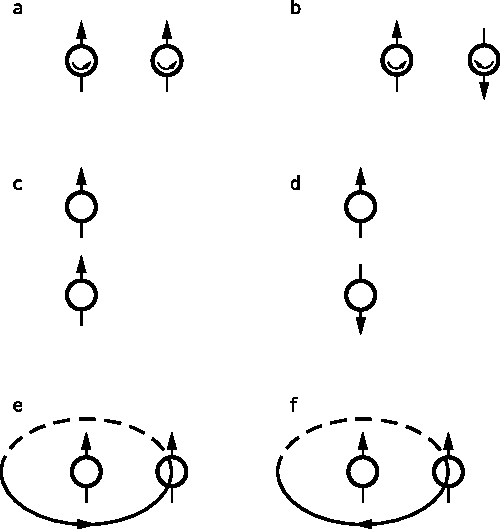
\includegraphics[width=0.7\linewidth]{fyz_fig183.pdf}
    \caption{Síla mezi dvěma protony závisí na všech možných parametrech. 
             (\cite[s.~148]{Feynman02}).}
    \label{fyz:fig183}
  \end{figure}

  \begin{figure}[ht!]  %\ref{fyz:fig184}
    \centering
    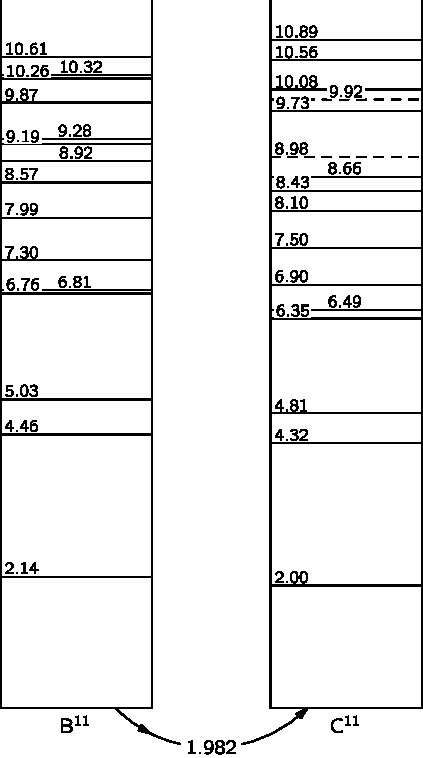
\includegraphics[width=0.7\linewidth]{fyz_fig184.pdf}
    \caption{Energetické hladiny jader \ce{^{11}B} a \ce{^{11}C} (hodnty udané v 
             \si{\mega\electronvolt}). Základní stav \ce{^{11}C} leží o 
             \SI{1.982}{\mega\electronvolt} výše než základní stav \ce{^{11}B}
             (\cite[s.~149]{Feynman02}).}
    \label{fyz:fig184}
  \end{figure}
  
\section{Energie v elektrostatickém poli}\label{fyz:IIchapVIsecV}

  \begin{figure}[ht!]  %\ref{fyz:fig185}
    \centering
    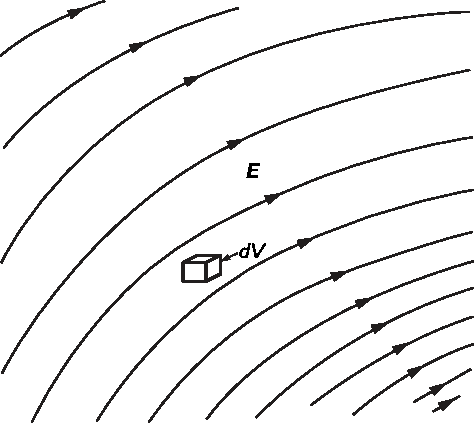
\includegraphics[width=0.7\linewidth]{fyz_fig185.pdf}
    \caption{Každý element objemu \(\dd{V} = \dd{x}\dd{y}\dd{z}\) v elektrickém  poli obsahuje 
    energii \(\varepsilon_0/2E^2\dd{V}\) 
             (\cite[s.~154]{Feynman02}).}
    \label{fyz:fig185}
  \end{figure}
  
\section{Energie bodového náboje}\label{fyz:IIchapVIsecVI}

%} %tikzset
%~~~~~~~~~~~~~~~~~~~~~~~~~~~~~~~~~~~~~~~~~~~~~~~~~~~~~~~~~~~~~~~~~~~~~~~~~~~~~~~~~~~~~~~~~~~~~~~~~~
\printbibliography[title={Seznam literatury}, heading=subbibliography]
\addcontentsline{toc}{section}{Seznam literatury}